\chapter*{Research Question 2}
\addcontentsline{toc}{chapter}{Research Question 2}
% Chapter for each research question
% how we validated it and proved it worked

\textit{What processes or algorithms need to be developed to filter or flag known instances of human interference from radio signal observations?}

\begin{itemize}
	\item Flag transmission signals identified by amateur radio enthusiasts from a local DXSpider server in recorded data.
  	\item Flag instances of natural radio interference such as lightning from the Blitzortung server in recorded data.
\end{itemize}

\section*{Flag Amateur Radio Enthusiast Transmissions}
\addcontentsline{toc}{section}{Flag Amateur Radio Enthusiast Transmissions}

\newglossaryentry{DXCluster}
{
	name={DXCluster},
	description={DXCluster - Number of DXServers connected together into a cluster, where amateur radio enthusiasts can share spotted instances of radio contact between each other},
	sort=DXCluster
}

%
\begin{figure}[!htb]
	\centering
	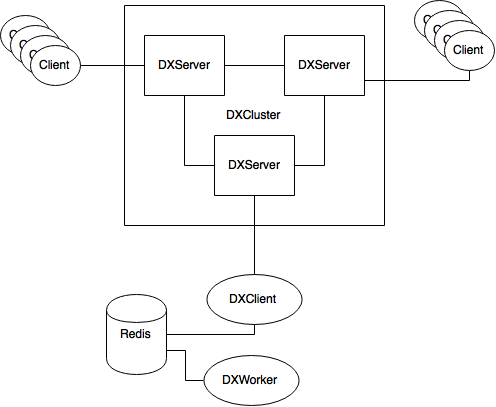
\includegraphics[width=8cm]{images/72}
	\caption{DXCluster Client Architecture}
	\label{fig:dxcluster_client_architecture}
\end{figure}
%

A DX server is a system which Amateur (Ham) Radio operators may use in order to inform one another in real time, about instances of radio signal transmissions from DX stations and other amateur radio stations. These DX Servers are often connected together to form a cluster. This allows many users from all over the world to communicate and share this information by connecting to the cluster. It is a rich source of identified human transmissions which often have the time, location and signal frequencies which were recorded. The data being shared is also often rigidly structured which greatly simplifies the task of implementing a software parsing solution \citep{koopman-07}. Table: \ref{tab:dxspider_data_packet} details the format of each packet of information shared on the DXCluster. 

%
\begin{table}
	\centering
	\begin{tabular}{p{4cm} l}
		\toprule
		Key & Sample Value\\ \midrule
		Call Sign of Spotter & DX de EA1MX: \\
		Frequency & 144364.0 \\
		DX Call Sign & TM64TDF \\
		Comment & IN73XK\textless TR\textgreater IN93OA tnx qso \\
		Time & 1623Z \\
		\bottomrule
	\end{tabular}
	\caption{Sample DXSpider Data Packet}
	\label{tab:dxspider_data_packet}
\end{table}
%
                   

A software client was developed in order to connect to a local server within the \gls{DXCluster}. The architecture diagram is shown in Figure: \ref{fig:dxcluster_client_architecture}. It was designed to gather all data from the cluster while filtering transmissions outside the frequency range currently being monitored by the telescope, and also filtering transmissions outside Europe. All signals which have been identified as being within the range being monitored, would be flagged and all related meta data for each transmission would be stored for processing at a later stage.


\subsection*{Methodology}
The aim of this experiment was to record 24 hours worth of data on the \gls{DXCluster} for signals originating in Europe within the frequency range being monitored by the SDRT system. The following methodology was followed during this experiment:

\begin{enumerate}
	\item Collect 24 hours worth of data using the \gls{DXCluster} Client developed
	\item Filter out all signals not originating in Europe
	\item Filter out all signals outside the target range of 18 MHz - 40 MHz
\end{enumerate}

The experiment was run for 24 hours, and during this time, 1984 transmissions were recorded on the \gls{DXCluster}. The data was filtered to only save transmissions originating from European countries, and also filtered further to only contain transmissions within the range being monitored by the SDRT namely 18 MHz - 40 MHz. This reduced the number of transmissions recorded to 209. The Figure: \ref{fig:dxcluster_country_barplot} shows a high level breakdown of the most popular countries for which transmissions originated from during the 24 hour period of monitoring. Figure \ref{fig:dxcluster_time_plot} shows this same data broken down by the hour it was collected and finally Figure: \ref{fig:dxcluster_frequency_plot} shows this data broken down by the radio frequency on which the transmission originated. As Figure: \ref{fig:dxcluster_frequency_plot} demonstrates, the majority of signals appear within narrow bands as is to be expected, as amateur radio enthusiasts operate in bands such as the 10M band for instance which corresponds with a frequency range of 28.000 MHz - 29.700 MHz, and then within channels inside this range.

%
\begin{figure}	
	\centering
	\begin{subfigure}[t]{8cm}
		\centering
		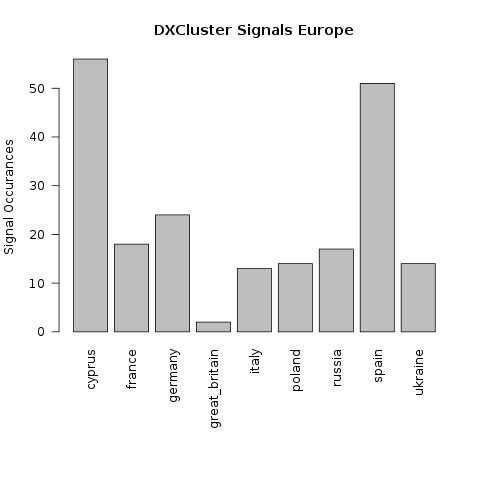
\includegraphics[width=5cm]{images/68}
		\caption{Top European countries represented in 24 hours}
		\label{fig:dxcluster_country_barplot}		
	\end{subfigure}
	\quad
	\begin{subfigure}[t]{5cm}
		\centering
		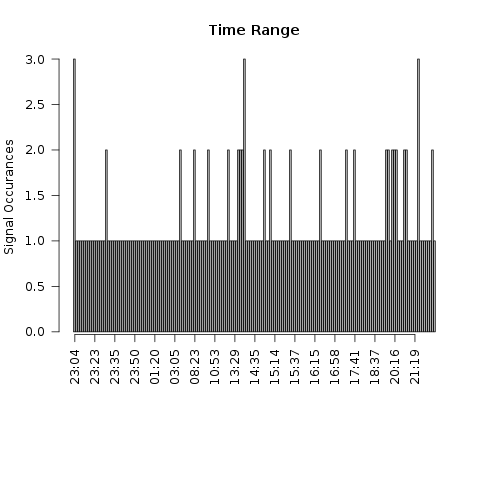
\includegraphics[width=5cm]{images/69}
		\caption{Time European signals occurred}
		\label{fig:dxcluster_time_plot}		
	\end{subfigure}
	\quad
	\begin{subfigure}[t]{5cm}
		\centering
		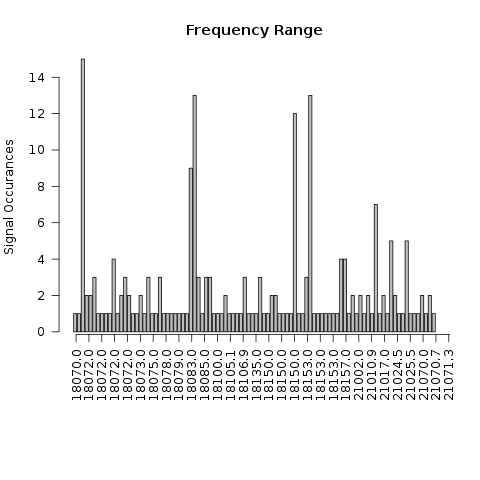
\includegraphics[width=5cm]{images/70}
		\caption{European signals within monitored frequency range}
		\label{fig:dxcluster_frequency_plot}
	\end{subfigure}
	\caption{DXCluster data}
	\label{fig:dxcluster_data}
\end{figure}
%

\section*{Flag Natural Emission Sources}
\addcontentsline{toc}{section}{Flag Natural Emission Sources}
The Blitzortung project operates an online service which displays global information about instances of lightning strikes in real time. \cite{blitzortung-14} provide the designs for a listening station which amateur enthusiasts can then build and operate. Each site can share information collected on local instances of lightning with the central server in real time \citep{blitzortung-14}. A software client was developed which can retrieve data on lightning strike occurrences from within Europe in 10 minute blocks from the Blitzortung server. Table: \ref{tab:blitzortung_data_packet} details the format of each Blitzortung data packet.

%
\begin{table}
	\centering
	\begin{tabular}{p{4cm} l}
		\toprule
		Key & Sample Value\\ \midrule
		Date & 2015-08-03 \\
		Time & 21:40:03.600511018 \\
		Latitude, Longitude,\\Elevation & pos;43.899106;20.438919;0 \\
		Unknown & str;0 \\
		Station ID & dev;14497 \\
		Confirming Stations &  sta;11;24;951,956,1313,1171,803 \\
		\bottomrule
	\end{tabular}
	\caption{Sample Blitzortung Data Packet}
	\label{tab:blitzortung_data_packet}
\end{table}
%

The Haversine function shown in Figure: \ref{fig:haversine_formula} provides the means to determine the distance between two points on a spherical surface, which Earth approximately is \citep{pineda-krch-10}. In this function, $\varphi$ corresponds with latitude, $\lambda$ corresponds with longitude and $R$ is the radius of the Earth. This function is used to measure the distance between the location of the SDRT listening site and each individual lightning strike data point. With this distance value, it is then possible to discard data points which originate further from the SDRT listening site than a chosen value such as 1000km.

%
\begin{figure}[here]
	\centering
	\begin{equation}
		a = sin^2\big(\frac{\Delta \varphi}{2}\big) + cos(\varphi_1) \times cos(\varphi_2) \times sin^2\big(\frac{\Delta \lambda}{2}\big)
	\end{equation}
	\begin{equation}
		c = 2arcsin\big(min(1,\sqrt{a})\big)
	\end{equation}
	\begin{equation}
		distance = R \times c
	\end{equation}
	\caption{Haversine Formula}
	\label{fig:haversine_formula}
\end{figure}
%

\subsection*{Methodology}
The following methodology was followed during this experiment:

\begin{enumerate}
	\item Collect 10 minutes of data using the Blitzortung Client developed
	\item Filter out all lightning strikes not originating in Europe
	\item Filter out all lightning strikes outside the target range of 1000km
\end{enumerate}


%
\begin{figure}	
	\centering
	\begin{subfigure}[t]{5cm}
		\centering
		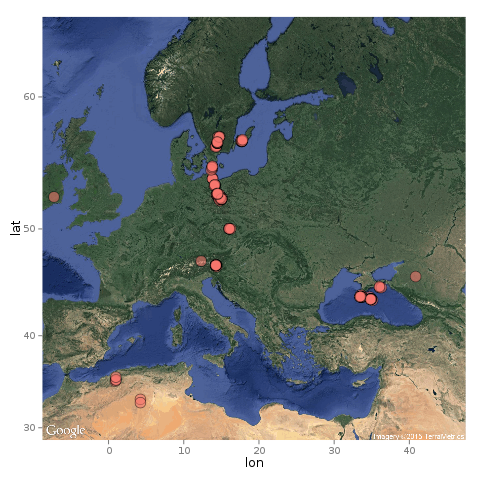
\includegraphics[width=5cm]{images/73}
		\caption{Lightning Strikes Above Europe}
		\label{fig:blitzortung_europe_plot}		
	\end{subfigure}
	\quad
	\begin{subfigure}[t]{5cm}
		\centering
		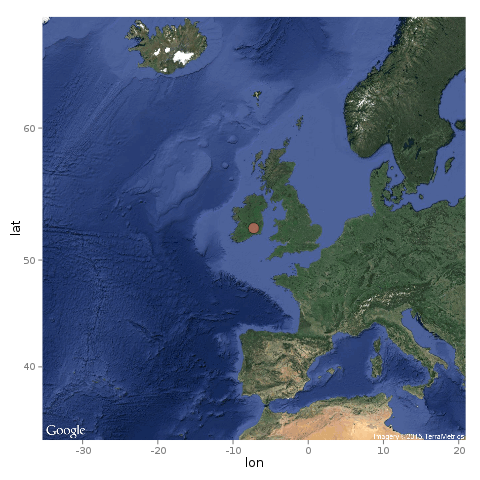
\includegraphics[width=5cm]{images/74}
		\caption{Strikes \textgreater 1000km filtered}
		\label{fig:blitzortung_europe_plot_filtered}
	\end{subfigure}
	\caption{Blitzortung data}
	\label{fig:blitzortung_europe_plot_both}
\end{figure}
%